\chapter{Flexible Diffusion for Arbitrary Conditioning}
\label{ch:flexible-diffusion}

% so far we've looked at conditioning on a fixed input
% for a lot of applications, it is more useful to be able to vary what we condition on
% in general this is very hard
% a minimal version is to be able to condition on anything that you're able to generate

% discuss test-time conditioning and its pitfalls
% so we will use an approach based on the learned conditional diffusion models from \cref{ch:conditional-diffusion}

So far in this thesis we have introduced both the diffusion models in both the conditional and unconditional forms. We've discussed the applications of conditional diffusion models to tasks including text-to-image, text-based image editing, and matrix factorisation. A similarity between these tasks is that we always knew in advance which data we wanted to condition on at test-time: for text-to-image we always condition on a text string; for text-based image editing we always condition on a text string and an input image; for matrix factorisation we always condition on the observed product matrix. In other words, we always knew during training what form the conditioning information $\rvy$ would take at test-time.

Our thesis in this work is that diffusion models can be made robust to cases where we do not know exactly what form $\rvy$ will take at test-time. There are many applications where this may be the case. For image inpainting, it is desirable to have a single inpainting model that can inpaint any pixels in an image depending on a user's requirements at test time. For video editing (or video generation from keyframes), a user might want to condition on every second frame, every tenth frame, only the first few frames, or so on. In the world modelling and planning example in \cref{fig:fdm-example-tasks}, we showed that conditioning a world model in different ways unlocked completely different capabilities and the ability to flexibly choose between these capabilities without retraining would be desirable.

In this chapter we propose the \textit{flexible} diffusion framework. Flexible diffusion models are trained to perform well on a variety of tasks, where different tasks require conditioning on a different type of conditioning information $\rvy$. Ideally we would like to train a diffusion model that could be trained once and then have it perform any conceivable conditioning task without requiring further training or the incorporation of new models. Clearly, having a model that can perform \textit{any} conceivable conditioning task is not possible: it wouldn't make sense to train a model on a dataset of images and then expect it to perform text-conditional image generation without ever having seen text data. Therefore given a domain with data $\rvx \sim \pdata(\cdot)$, we will focus on tasks that can be described as conditioning on a subset of the dimensions of $\rvx$. In particular we will describe what $n_\rvy$ dimensions to condition on as a set of integer indices $\gY = \{ y_1, \ldots, y_{n_\rvy} \}$. We will then define $\rvy$ as a vector in $\mathbb{R}^{n_\rvy}$ in the $i$th element is equal to $\rvx[y_i]$. Different $\gY$ correspond to different conditional generation tasks, with the conditional generation task being to generate samples from
\begin{equation} \label{eq:flexible-diffusion-target}
    \pdata(\rvx | \rvy, \gY)
\end{equation}
where $\gY = \{ y_1, \ldots, y_{n_\rvy} \}$ and $\rvy = [ \rvx[y_1], \ldots, \rvx[y_{n_\rvy}] ]$. In other words, each conditional generation task is to sample data conditioned on observed values and with knowledge of the index of each observed value.

In the following chapters we will consider several variations of this task. In \cref{ch:fdm}, we will define a model that only samples a subset of the dimensions in the original data. In this case we will modify \cref{eq:flexible-diffusion-target} to also condition on $\gX$, the indices of dimensions we wish to generate and samples $\rvx$ will contain only those only $|\gX|$ elements. In \cref{ch:tddm} we will explore the case where the data has varying dimensionality and $\pdata(\rvx | \rvy, \gY)$ is a trans-dimensional distribution from which different samples can have different dimensionality. In this case, conditioning on $\gY$ also implies conditioning on $\rvx$ having at least as many dimensions as suggested by the largest index in $\gY$.

We will for now consider just the simpler case described by the target distribution in \cref{eq:flexible-diffusion-target}. We will denote the approximation of this target from a flexible diffusion model $p_\theta(\rvx|\rvx,\gY)$. To train this flexible diffusion model we use the objective
% To, we write the flexible diffusion objective in the same way as the conditional diffusion objective in \cref{eq:cond-diffusion-loss},
\begin{align} \label{eq:flexible-diffusion-loss}
    \mathcal{L}_\text{ISM}(\theta) &= \int_{\sigma_\text{min}}^{\sigma_\text{max}} \lambda^\rvx(\sigma) \EX_{u(\gY)q(\rvx, \rvx_\sigma)\delta(\rvy|\rvx,\gY)} \left[ 
    || \rvx_\theta(\rvx_\sigma, \rvy, \sigma, \gY) - \rvx ||_2^2 \right] \mathrm{d}\sigma.
\end{align}
Note that this flexible diffusion objective is very similar to the conditional diffusion objective in \cref{eq:cond-diffusion-loss}, with the differences being as follows. First, we now have an expectation over $\gY \sim u(\cdot)$. We will call $u(\gY)$ our \textit{training task} distribution and it is up to the developer of a flexible diffusion model to construct it. Second, we now sample $\rvy$ from $\delta(\rvy|\rvx,\gY)$, a Dirac distribution on $\rvy = [ \rvx[y_1], \ldots, \rvx[y_{n_\rvy}] ]$, instead of sampling it from a dataset. Note that another consequence of this way of sampling $\rvy$ is that it may now have varying dimensionality between different training examples: its dimensionality $n_\rvy$ can now in principle be anywhere between zero and the dimensionality of $\rvx$. Third, we now pass $\gY$ as an extra input into the neural network parameterising $\rvx_\theta(\rvx_\sigma, \rvy, \sigma, \gY)$. We will describe how exactly $\gY$ is fed into the neural network for each task in this dissertation as we get to it.

Finally, note that we write the flexible diffusion objective in  \cref{eq:flexible-diffusion-loss} as if we are expecting $\rvx_\theta(\rvx_\sigma, \rvy, \sigma, \gY)$ to contain predictions for all dimensions of $\rvx$, even dimensions that are specified in $\gY$ and so observed in $\rvy$. In practice a neural network is not needed to make predictions for these dimensions; we can manually implement functionality that copies these values from the input $\rvy$ into the output $\rvx_\theta(\rvx_\sigma, \rvy, \sigma, \gY)$. The squared-error loss for such dimensions will then always be zero. The fact that we include them in the squared-error in \cref{eq:flexible-diffusion-loss} is therefore not important in practice.

We end this section with an intuitive example of a task where flexible conditioning is required: solving Sudoku puzzles~\citep{weilbach2023graphically}. A Sudoku is a $n^2 \times n^2$ grid of integers with each one taking a value in $\{1,\ldots,n^2\}$. Most commonly, $n$ is set to three so the grid has size $9 \times 9$. There are three types of constraint required for a Sudoku to be valid: no value can appear more than once within the same row of the grid; no value can appear more than once within the same column; and no value can appear more than once within any of the $n^2$ $n \times n$ sub-grids that make up the grid. Sudoku puzzles are puzzles in which the player is given a Sudoku with many values missing. The player is then required to fill in the missing values. Most puzzles are constructed to have a single solution, but if the values in sufficiently few cells are given then multiple solutions can be possible. We can frame solving Sudokus as a conditional generative modelling problem if we have a data distribution $\pdata(\rvx)$ that places probability mass over all complete and valid Sudoku grids.\footnote{Fortunately this distribution is efficient to sample from. See implementation at \url{https://turtletoy.net/turtle/5098380d82}.} The set of observed indices $\gY$ denotes which cells the user is given values for, and the user must infer the values for all cells not in $\gY$. The cells whose values are given as clues vary between different Sudoku puzzles, and so training a conditional generative model that can solve any given Sudoku puzzle means training a flexible generative model. We refer to \citet{weilbach2023graphically} for further details of this model.

In the next sections we describe how flexible diffusion models can be adapted for long video generation (\cref{ch:fdm}) and for generation of varying-length videos as well as data like molecules (\cref{ch:tddm}). Finally, in \cref{ch:cigcvae}, we will transfer these ideas to the variational auto-encoder framework and construct a  flexible generative model for the image inpainting problem.

\begin{figure}
    \centering
    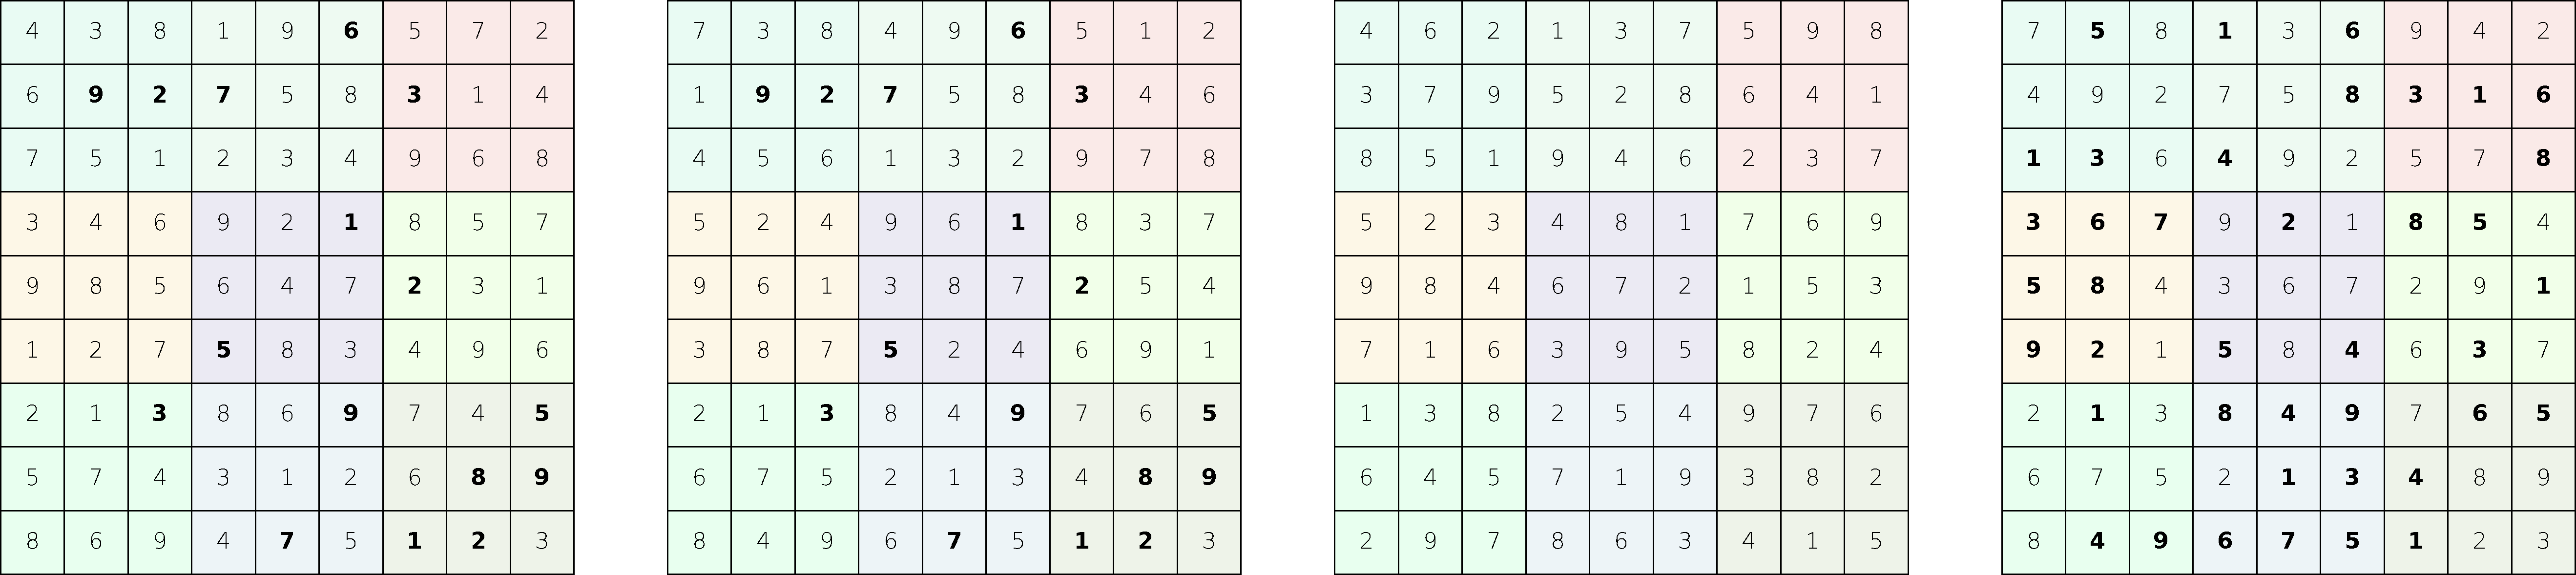
\includegraphics[width=\textwidth]{figs/thesis/sudoku_panel.pdf}
    \caption{Sudoku puzzles solved by a flexible generative model. Observed numbers (i.e. those that form part of $\rvy$) are shown in bold. The observed numbers are the same for the leftmost two Sudokus but multiple solutions exist, and we show that the generative model is able to find two different solutions. In the third Sudoku from the left, no numbers were observed. This corresponds to the task with $\gY = \{\}$. The training task distribution $u(\gY)$ covered such tasks and so this flexible generative model is capable of unconditional generation as shown. }
    \label{fig:sudoku-panel}
\end{figure}